\section{ジッターの評価}
これまでの測定から、立ち上がり時間$t_{\rm{r}}$、60%から40%の波高の差$S$、ノイズ$\sigma_{\rm{n}}$を求めることができた。
この測定結果と 式\ref{eq_Jitter_1} を用いて、PINとLGADのジッター$\sigma_{\rm{j}}$を求めた。
%\begin{equation}
%    \sigma_j = \frac{\sigma_n}{|\frac{dV}{dt}|} = \frac{\sigma_n}{|\frac{S}{t_r}|} = \frac{t_r}{|\frac{S}{\sigma_n}|}
%    \label{eq_Jitter}
%\end{equation}
 図\ref{fg:JittervsBias} にLGADとPINのジッターの電圧依存性を示す。
横軸が電圧で縦軸がジッターである。また、青点がPIN、赤点がLGADの測定データである。
PINのジッターは電圧が大きくなると減少し、その減少量は印加電圧が大きくなるにつれて小さくなり、およそ42 ps になることがわかった。
PINの立ち上がり時間とノイズは電圧に依存せずに一定であるため、空乏層の拡大による信号の大きさの増加がジッターの減少に影響していると考える。
LGADのジッターは電圧を上げるほど小さくなり、最小値が198 V でおよそ1.9 ps であった。
LGADは印加電圧の増加により、立ち上がり時間が早くなり、信号の大きさが増加するため、ジッターが小さくなると考える。
また200Vでは、電子雪崩によってノイズが非常に大きくなる影響によって、少しだけ増加することがわかった。

\begin{figure}[h]
    \centering
    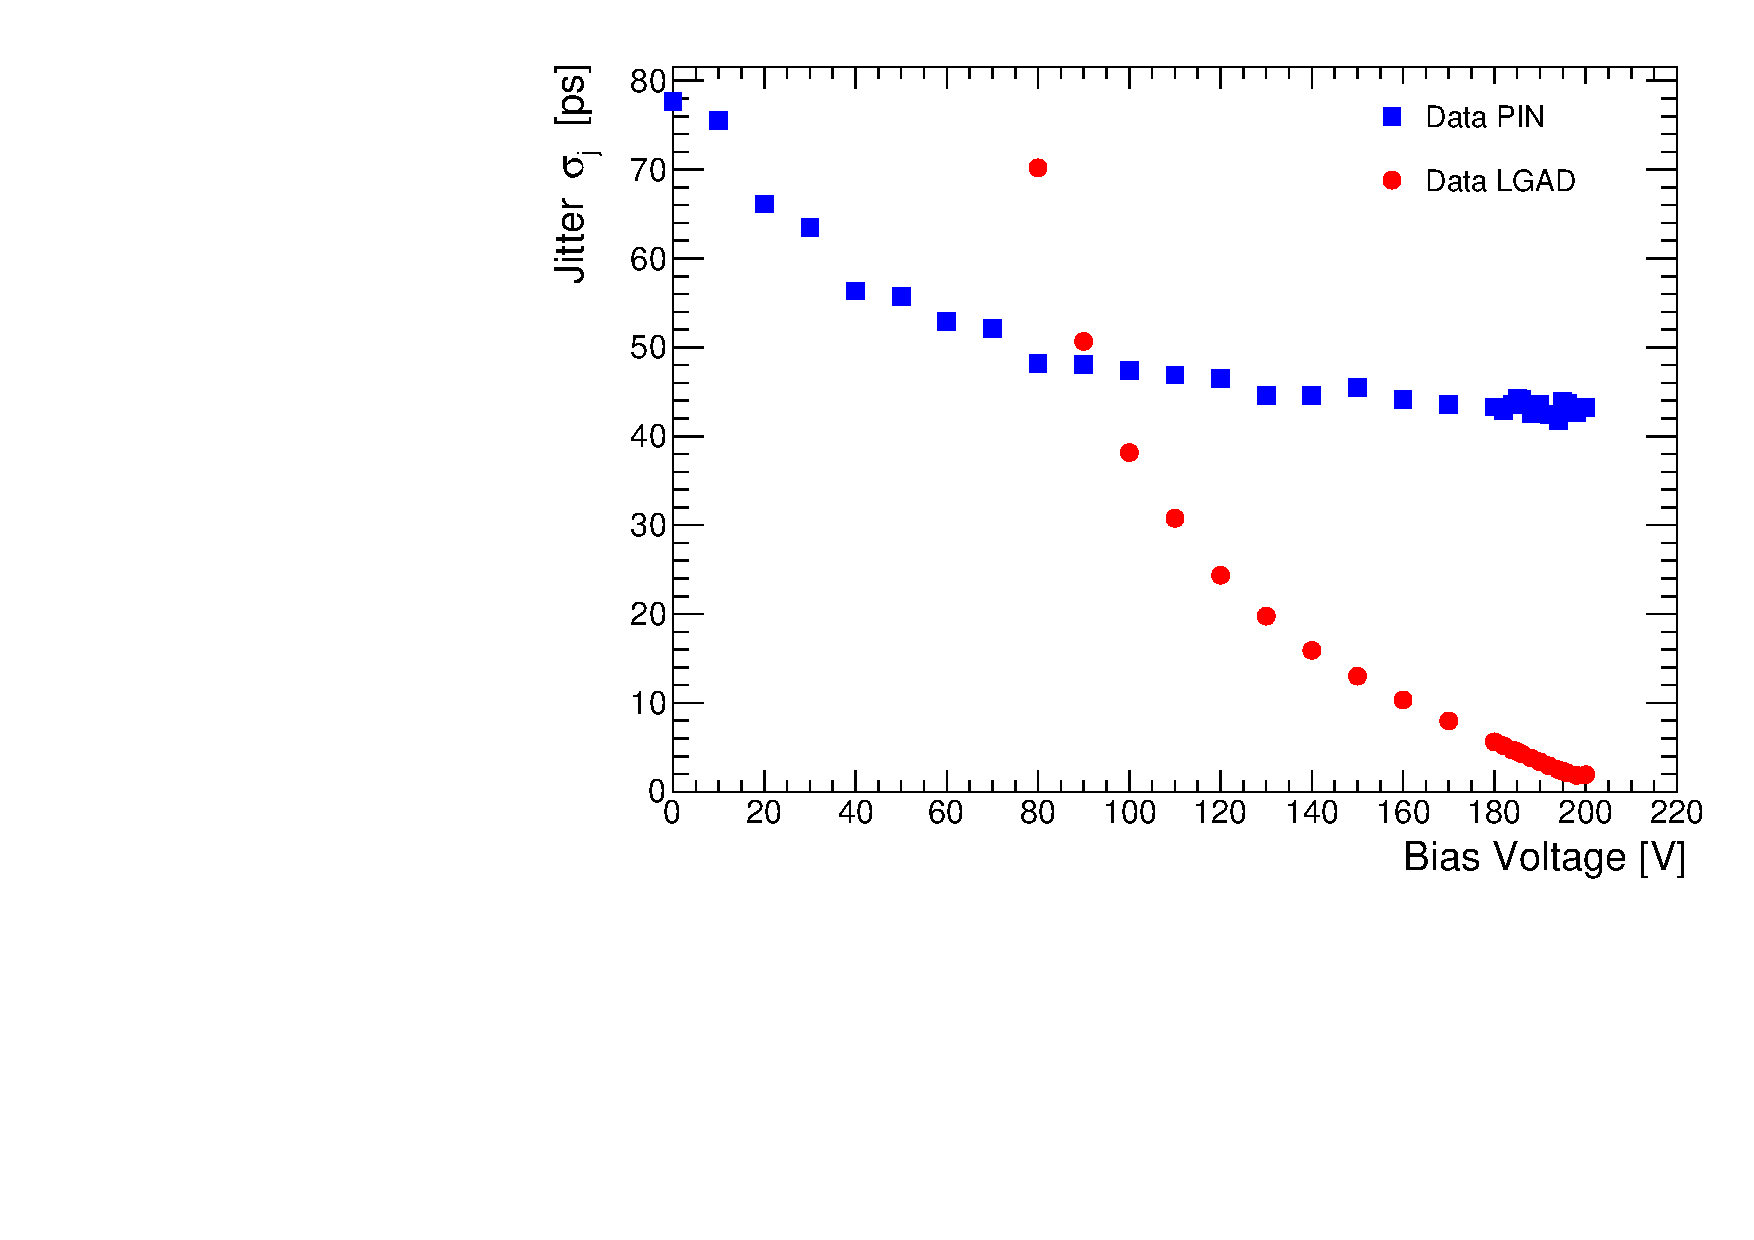
\includegraphics[width=10cm]{fig/graph/JittervsVoltage.pdf}
    \caption[AC-LGAD検出器のジッターの電圧依存性]{AC-LGAD検出器のジッターの電圧依存性\\横軸が電圧で縦軸がジッター、赤点がLGADで青点がPINの測定点}
    \label{fg:JittervsBias}
\end{figure}

さらに、図\ref{fg:Jitter_TresovsBias} に、LGADのジッター$\sigma_{\rm{j}}$とレーザー測定から求めた時間分解能$\sigma_{\rm{t}}$の増幅率依存性を示す。
横軸が増幅率で縦軸がジッターと時間分解能である。青点が時間分解能で赤点がジッターのデータ点である。
時間分解能は増幅率が大きくなると悪化するのに対して、ジッターは増幅率が大きくなると減少していることがわかる。
ジッターと時間分解能は一致せず、ジッターのみでは説明できない時間分解能の悪化が見られる
ことがわかった。
%実際にはノイズの悪化よりも、信号の大きさの増加が支配的であるため、ジッターは増幅率が大きくなると減少する。そのため、ノイズの増加が時間分解能の悪化の原因ではないことがわかった。
%レーザーを用いた測定では、タイムウォーク$\sigma_{tw}$とランダウノイズ$\sigma_L$の影響がほとんどないため、
そのため、AC-LGAD検出器の時間分解能は、ジッター、タイムウォーク、ランダウノイズに加わる要因があり、特に増幅率が大きい時にその効果が顕著であることがわかった。

\begin{figure}[h]
    \centering
    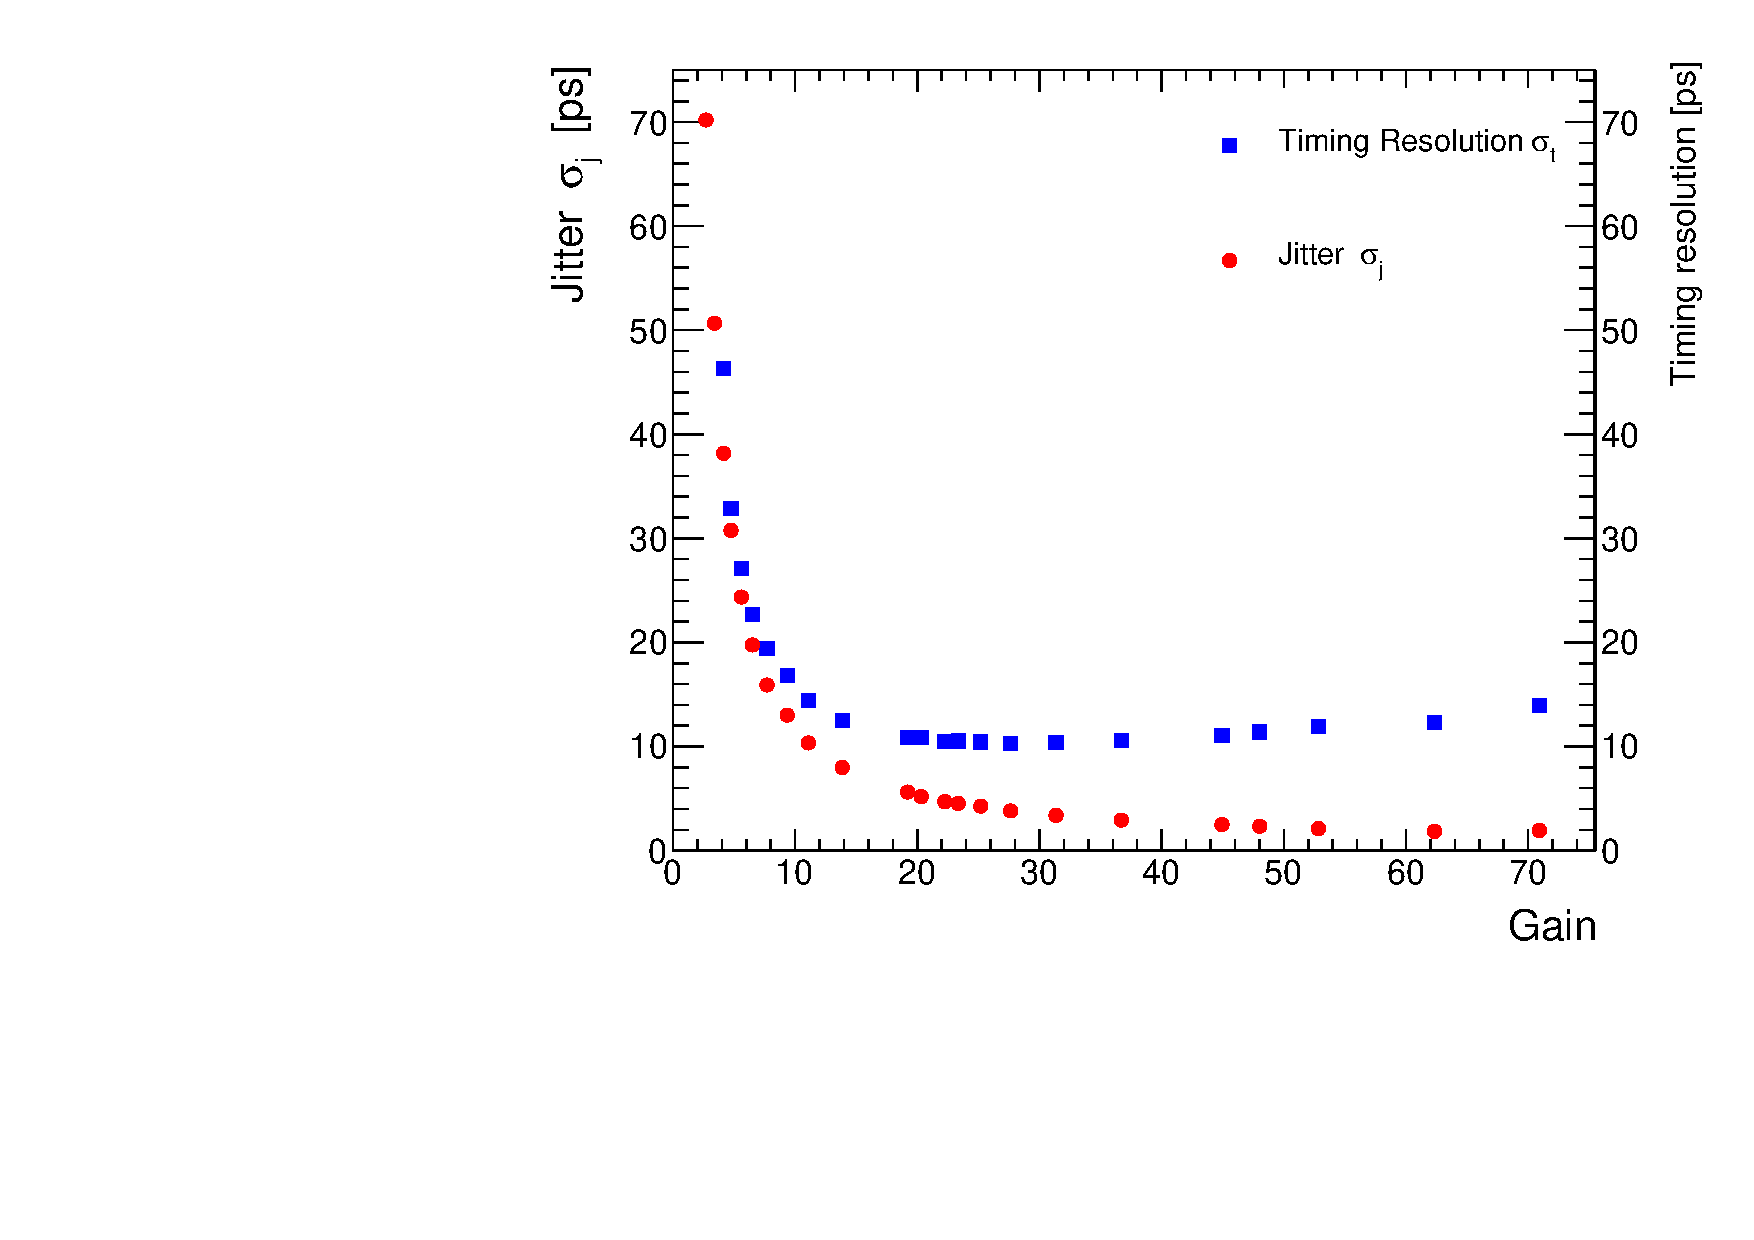
\includegraphics[width=10cm]{fig/graph/Treso&JittervsGain.pdf}
    \caption[AC-LGAD検出器の時間分解能とジッターの増幅率依存性]{AC-LGAD検出器の時間分解能とジッターの増幅率依存性\\横軸が増幅率で縦軸がジッターと時間分解能、青点が時間分解能で赤点がジッターのデータ点}
    \label{fg:Jitter_TresovsBias}
\end{figure}

時間分解能からジッターを引くことで、時間分解能を悪くする要因への理解を進めた。
図\ref{fg:Treso_JittervsGain_Minus} にその結果を示す。縦軸が時間で横軸が増幅率である。時間分解能が悪くなる様子を見るために、時間スケールを0〜20 psに変更した。
青点が時間分解能で赤点がジッター、ピンクの点が時間分解能とジッターの差についてである。
増幅率が小さい領域では、時間分解能とジッターの差は増幅率が上昇とともに減少し、増幅率が15 倍以上の領域では、増幅率の増加と共に上昇することがわかった。
時間分解能とジッターの差の最小値がおよそ15〜20 倍の領域で約9 psあるということが、レーザーの10 ps未満のタイミングジッタの影響を示していると考える。

時間分解能とジッターの差の最小値9.34 psをレーザーのタイミングジッターとして、その影響を差し引いた結果を 図\ref{fg:Treso_JittervsGain_Minus} の緑点に示す。
緑点が時間分解能を悪化させる要素である、増幅率が大きくなることで増加する過剰ノイズの様子を示していると考える。
過剰ノイズは増幅率がおよそ35 倍以上でジッターに対して支配的になることがわかった。
以上の結果と第3章の時間分解能が良い増幅率が20〜35倍という結果から、時間分解能が良い増幅率では過剰ノイズの影響が小さいと考えられる。

\begin{figure}[h]
    \centering
    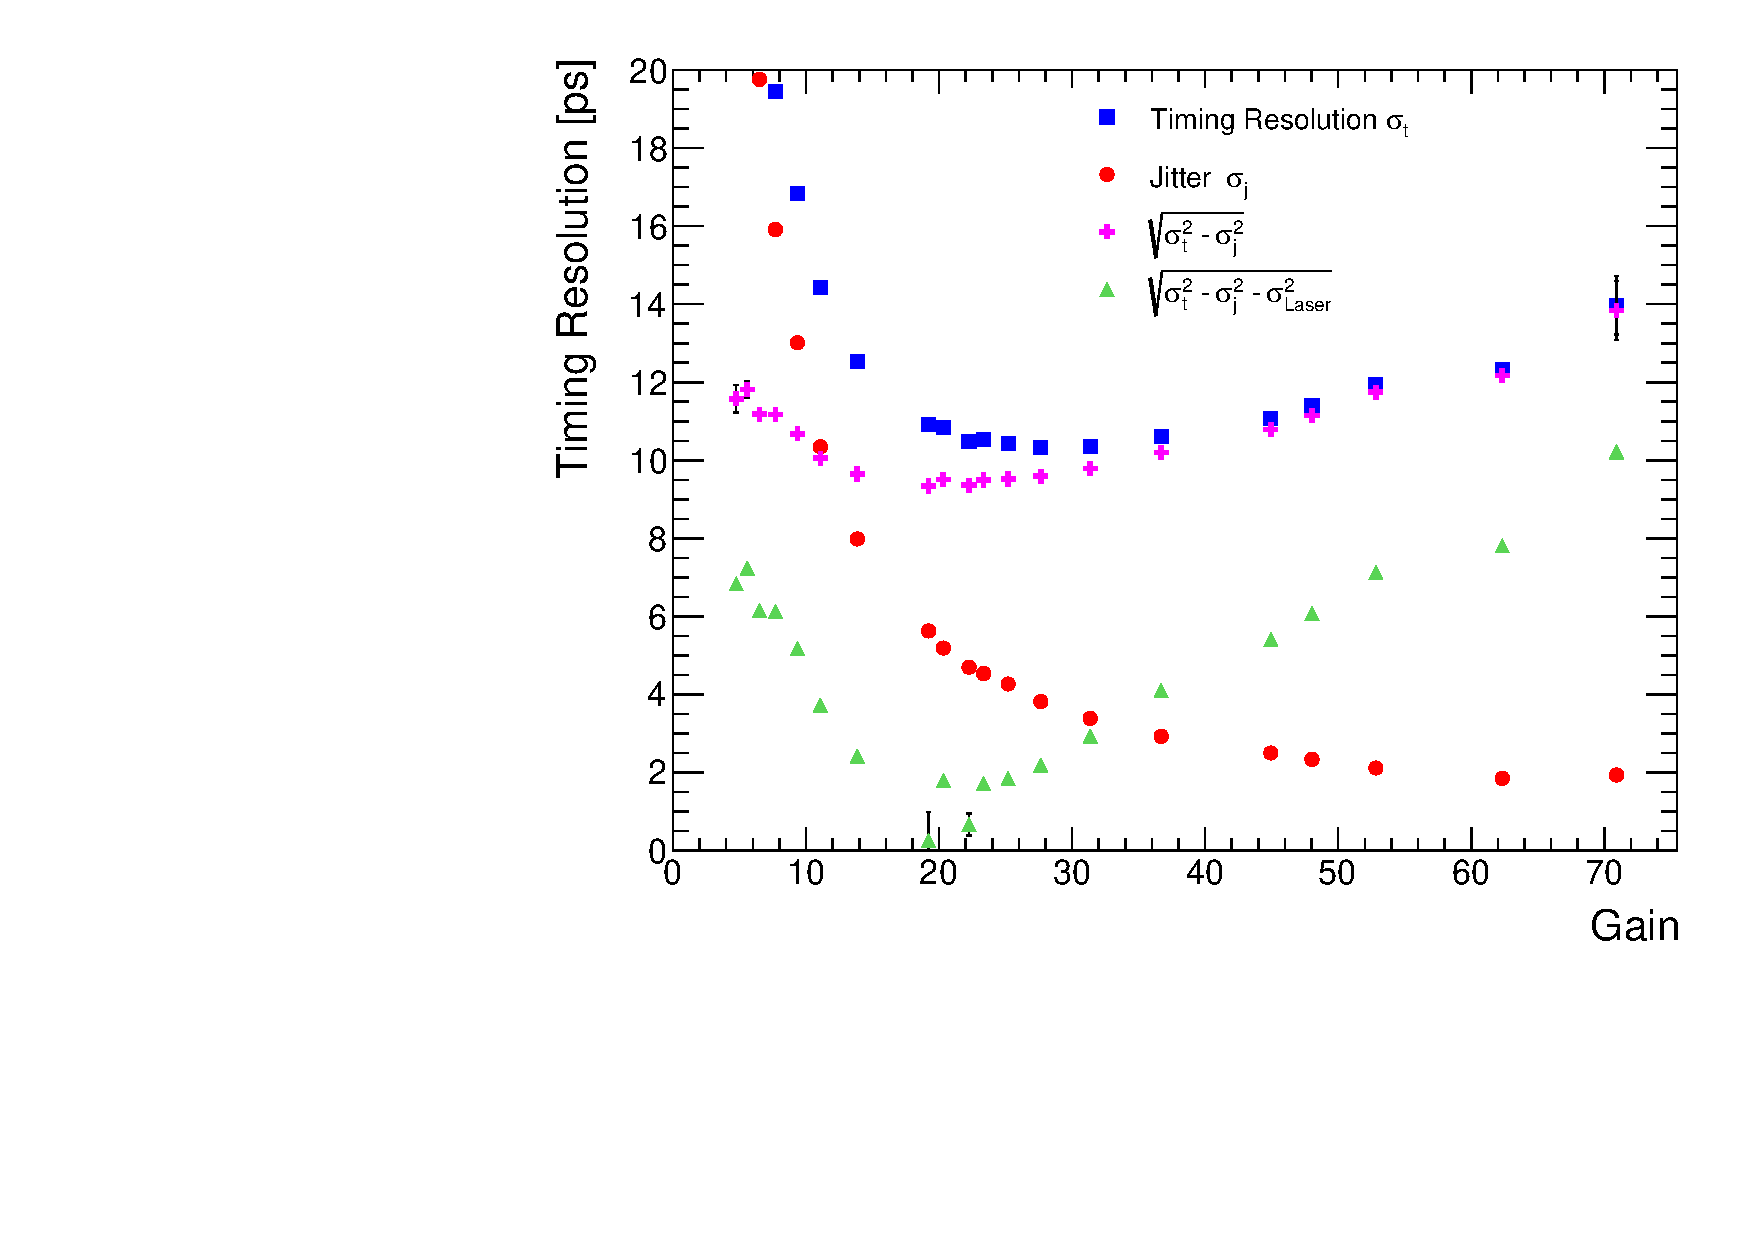
\includegraphics[width=10cm]{fig/graph/Jitter_Treso_MultivsGain.pdf}
    \caption[AC-LGAD検出器の時間分解能とジッターとその差の増幅率依存性]{AC-LGAD検出器の時間分解能とジッターとその差の増幅率依存性\\横軸が増幅率で縦軸がジッターと時間分解能、青点が時間分解能で赤点がジッター、ピンクの点が時間分解能とジッターの差、緑点がピンク点からレーザーのタイミングジッターを差し引いた結果}
    \label{fg:Treso_JittervsGain_Minus}
\end{figure}


